\documentclass{beamer}

\usepackage{tikz}
\usepackage{ngerman}
\usepackage{listings}
\usepackage{graphicx}

\usepackage{py_vortrag}


% title
\title{Einf"uhrung in Python}

\date{Februar 2011}

\author{Rebecca Breu}

\institute
{
 Verteilte Systeme und Grid-Computing \\
 JSC\\
 Forschungszentrum J"ulich
}


\begin{document}

\AtBeginPart
{
  \begin{frame}
  \titlepage
  \end{frame}

  \begin{frame}{Inhalt --- \insertpart}
  \tableofcontents
  \end{frame}
}


\AtBeginSection[]
{
   \begin{frame}{\insertsection}
       \tableofcontents[currentsection]
   \end{frame}
}


\begin{frame}
\titlepage
\end{frame}

\begin{frame}{Inhalt}
\begin{columns}[t]

\begin{column}{0.4\textwidth}
  Teil 1:\\[3mm]
  \tableofcontents[part=1]
\end{column}

\begin{column}{0.6\textwidth}
  Teil 2:\\[3mm]
  \tableofcontents[part=2]
  \vspace{7mm}
  Teil 3:\\[3mm]
  \tableofcontents[part=3]
\end{column}

\end{columns}
\end{frame}


\part{Teil 1}

\section{Einf"uhrung}

\begin{frame}{Was ist Python?}
\alert{Python:} dynamische Programmiersprache, welche verschiedene Programmierparadigmen unterst"utzt:
\begin{itemize}
\item prozedurale Programmierung
\item objektorientierte Programmierung
\item funktionale Programmierung
\end{itemize}
Standard: Python-Bytecode wird im Interpreter ausgef"uhrt ("ahnlich Java)\\
$\rightarrow$ \alert{plattformunabh"angiger Code}
\end{frame}

\begin{frame}{Warum Python?}
\begin{itemize}
\item Syntax ist klar, leicht zu lesen \& lernen (fast Pseudocode)
\item intuitive Objektorientierung
\item volle Modularit"at, hierarchische Pakete
\item Fehlerbehandlung mittels Ausnahmen
\item dynamische, \glqq High Level\grqq-Datentypen
\item umfangreiche Standard-Bibliothek f"ur viele Aufgaben
\item einfache Erweiterbarkeit durch C/C++, Wrappen von C/C++-Bibliotheken
\end{itemize}
\alert{Schwerpunkt: Programmiergeschwindigkeit!}
\end{frame}

\begin{frame}{Ist Python schnell genug?}
\begin{itemize}
\item f"ur rechenintensive Algorithmen: evtl. besser Fortran, C, C++ 
\item f"ur Anwenderprogramme: Python ist schnell genug!
\item Gro"steil der Python-Funktionen sind in C geschrieben
\item Performance-kritische Teile k"onnen jederzeit in C/C++ ausgelagert werden
\item erst analysieren, dann optimieren!
\end{itemize}
\end{frame}

\begin{frame}[fragile]{Hallo Welt!}
\begin{lstlisting}[style=Python]
#!/usr/bin/env python

# Dies ist ein Kommentar
print "Hallo Welt!"
\end{lstlisting}
\begin{lstlisting}[style=Shell]
$ python hallo_welt.py
Hallo Welt!
$
\end{lstlisting}%$
\begin{lstlisting}[style=Shell]
$ chmod 755 hallo_welt.py
$ ./hallo_welt.py
Hallo Welt!
$
\end{lstlisting} %$
\end{frame}

\begin{frame}[fragile]{Hallo User}
\begin{lstlisting}[style=Python]
#!/usr/bin/env python

name = raw_input("Wie heisst du? ")
print "Hallo", name
\end{lstlisting}
\begin{lstlisting}[style=Shell]
$ ./hallo_user.py
Wie heisst du? Rebecca
Hallo Rebecca
$
\end{lstlisting}
\end{frame}

\begin{frame}{Starke und dynamische Typisierung}
\alert{Starke Typisierung:}
\begin{itemize}
\item Objekt ist genau von einem Typ! String ist immer String, \texttt{int} immer \texttt{int}
\item Gegenbeispiele: PHP, C: \texttt{char} kann als \texttt{short} betrachtet werden, \texttt{void~*} kann alles sein
\end{itemize}
\alert{Dynamische Typisierung: }
\begin{itemize}
\item keine Variablendeklaration
\item Variablennamen k"onnen nacheinander unterschiedliche Datentypen zugewiesen werden
\item Erst zur Laufzeit werden Eigenschaften eines Objekts untersucht
\end{itemize}
\end{frame}

\begin{frame}[fragile]{Starke und dynamische Typisierung}
\begin{lstlisting}[style=Python]
zahl = 3
print zahl, type(zahl)
print zahl + 42
zahl = "3"
print zahl, type(zahl)
print zahl + 42
\end{lstlisting}
\begin{lstlisting}[style=Shell]
3 <type 'int'>
45
3 <type 'str'>
Traceback (most recent call last):
  File "test.py", line 6, in ?
    print zahl + 42
TypeError: cannot concatenate 'str' and 
'int' objects
\end{lstlisting}
\end{frame}

\begin{frame}[fragile]{Interaktiver Modus}
Der Interpreter kann im interaktiven Modus gestartet werden:
\begin{lstlisting}[style=Shell]
$ python
Python 2.6 (r26:66714, Feb  3 2009, 20:52:03) 
[GCC 4.3.2] on linux2
Type "help", "copyright", "credits" or ...
>>> print "hallo welt"
hallo welt
>>> a = 3 + 4
>>> print a
7
>>> 3 + 4
7
>>>
\end{lstlisting} %$
\end{frame}

\begin{frame}{Dokumentation}
Online-Hilfe im Interpreter:
\begin{itemize}
\item \alert{\lstinline{help()}}: allgemeine Hilfe zu Python
\item \alert{\lstinline{help(obj)}}: Hilfe zu einem Objekt, z.B. einer Funktion oder einem Modul
\item \alert{\lstinline{dir()}}: alle belegten Namen 
\item \alert{\lstinline{dir(obj)}}: alle Attribute eines Objekts
\end{itemize}
\vspace{5mm}
Offizielle Dokumentation: \href{http://docs.python.org/}{http://docs.python.org/}
\end{frame}

\begin{frame}[fragile]{Dokumentation}
\begin{lstlisting}[style=Shell]
>>> help(dir)
Help on built-in function dir:
...
>>> a = 3
>>> dir()
['__builtins__', '__doc__', '__file__', 
'__name__', 'a']
>>> help(a)
Help on int object:
...
\end{lstlisting}
\end{frame}


\section{Datentypen I}

\begin{frame}[fragile]{Numerische Datentypen}
\begin{itemize}
\item \alert{\texttt{int}}: entspricht \texttt{long} in C
\item \alert{\texttt{long}}: unbegrenzter Wertebereich
\item \alert{\texttt{float}}: enspricht \texttt{double} in C 
\item \alert{\texttt{complex}}: komplexe Zahlen
\end{itemize} 
\begin{lstlisting}[style=Python]
a = 1
b = 1L
c = 1.0; c = 1e0
d = 1 + 0j
\end{lstlisting}
\vspace{3mm}
Integers werden bei Bedarf automatisch in long umgewandelt! 
\end{frame}

\begin{frame}{Operatoren auf Zahlen}
\begin{itemize}
\item \alert{Grundrechenarten}: \texttt{+}, \texttt{-}, \texttt{*}, \texttt{/}
\item Div- und Modulo-Operator: \texttt{//}, \hspace{1mm}\texttt{\%}, \hspace{1mm}\texttt{divmod(x, y)}
\item \alert{Betrag}: \texttt{abs(x)}
\item \alert{Runden}: \texttt{round(x)}
\item Konvertierung: \texttt{int(x)}, \texttt{long(x)}, \texttt{float(x)}, \texttt{complex(re~[, im=0])}
\item Konjugierte einer komplexen Zahl: \texttt{x.conjugate()}
\item \alert{Potenzen}: \texttt{x ** y}, \hspace{1mm}\texttt{pow(x, y)}
\end{itemize}
Ergebnis einer Verkn"upfung unterschiedlicher Datentypen ist vom Typ des \glqq gr"o"seren\grqq{} Datentyps.
\end{frame}

\begin{frame}[fragile]{Strings}
Datentyp: \alert{\lstinline{str}}
\begin{itemize}
\item \lstinline{s = 'spam'}, \lstinline{s = "spam"}
\item Mehrzeilige Strings: \lstinline{s = """spam"""}
\item keine Interpretation von Escape-Sequenzen: \lstinline{s = r"spam"}
\item Strings aus anderen Datentypen erzeugen: \lstinline{str(1.0)}
\end{itemize}
\begin{lstlisting}[style=Shell]
>>> print "sp\nam"
sp
am
>>> print r"sp\nam"
sp\nam
>>> s = """hallo
... welt"""
>>> print s
hallo
welt
\end{lstlisting}
\end{frame}

\begin{frame}{String-Methoden}
\begin{itemize}
\item Vorkommen von Substrings z"ahlen: \lstinline{s.count(sub [, start[, end]])}
\item beginnt/endet s mit einem Substring? \lstinline{s.startswith(sub[, start[, end]])}, \lstinline{s.endswith(sub[, start[, end]])}
\item s in Gro"s-/Kleinbuchstaben: \lstinline{s.upper()}, \lstinline{s.lower()}
\item Leerraum entfernen: \lstinline{s.strip([chars])}
\item an Substrings trennen: \lstinline{s.split([sub [,maxsplit]])}
\item Position eines Substrings finden: \lstinline{s.index(sub[, start[, end]])}
\item einen Substring ersetzen: \lstinline{s.replace(old, new[, count])}
\end{itemize}
Weitere Methoden: \lstinline{help(str)}, \lstinline{dir(str)}
\end{frame}

\begin{frame}{Listen}
Datentyp: \alert{\lstinline{list}}
\begin{itemize}
\item \lstinline{s = [1, "spam", 9.0, 42]}, \;\lstinline{s = []}
\item \alert{Element anh"angen}: \lstinline{s.append(x)}
\item um zweite Liste erweitern: \lstinline{s.extend(s2)}
\item Vorkommen eines Elements z"ahlen: \lstinline{s.count(x)}
\item Position eines Elements: \lstinline{s.index(x[, min[, max]])}
\item Element an Position einf"ugen: \lstinline{s.insert(i, x)}
\item Element an Position l"oschen und zur"uckgeben: \lstinline{\s.pop([i])}
\item \alert{Element l"oschen}: \lstinline{s.remove(x)}
\item Liste umkehren: \lstinline{s.reverse()}
\item \alert{Sortieren}: \lstinline{s.sort([cmp[, key[, reverse]]])}
\item Summe der Elemente: \lstinline{sum(s)}
\end{itemize}
\end{frame}

\begin{frame}{Operationen auf Sequenzen}
Stings und Listen haben viel gemeinsam: Sie sind \alert{Sequenzen}.
\begin{itemize}
\item Ist ein Element in s enhalten/nicht enthalten?\\
 \lstinline{x in s}, \lstinline{x not in s}
\item Sequenzen aneinanderh"angen: \lstinline{s + t}
\item Sequenzen vervielf"altigen: \lstinline{n * s}, \lstinline{s * n}
\item \alert{i-tes Element}: \lstinline{s[i]}, von hinten: \lstinline{s[-i]}
\item Subsequenz: \lstinline{s[i:j]}, mit Schrittweite k: \lstinline{s[i:j:k]}
\item Subsequenz von Anfgang/bis Ende: \lstinline{s[:-i]}, \lstinline{s[i:]}, \lstinline{s[:]}
\item \alert{L"ange}: \lstinline{len(s)}
\item kleinstes/gr"o"stes Element: \lstinline{min(s)}, \lstinline{max(s)}
\item Zuweisungen: \lstinline{(a, b, c) = s} \\
$\rightarrow$ \lstinline{a = s[0]}, \lstinline{b = s[1]}, \lstinline{c = s[2]}
\end{itemize}
\end{frame}

\begin{frame}[fragile]{Sequenzen}
\begin{itemize}
\item Auch eine Sequenz: Datentyp \alert{\texttt{tuple}}: a = (1, 2, 3)
\item Listen sind ver"anderbar
\item Strings und Tupel sind nicht ver"anderbar
\begin{itemize}
\item Keine Zuweisung \lstinline{s[i] = ...}
\item Kein Anh"angen und L"oschen von Elementen
\item Funktionen wie \texttt{upper} liefern einen neuen String zur"uck!
\end{itemize}
\end{itemize}
\begin{lstlisting}[style=Shell]
>>> s1 = "spam"
>>> s2 = s1.upper()
>>> s1
'spam'
>>> s2
'SPAM'
\end{lstlisting}
\end{frame}

\begin{frame}[fragile]{Referenzen}
\begin{itemize}
\item In Python ist alles eine Referenz auf ein Objekt!
\item Vorsicht bei Zuweisungen:
\end{itemize}
\begin{lstlisting}[style=Shell]
>>> s1 = [1, 2, 3, 4]
>>> s2 = s1
>>> s2[1] = 17
>>> s1
[1, 17, 3, 4]
>>> s2
[1, 17, 3, 4]
\end{lstlisting}
Flache Kopie einer Liste: \lstinline{s2 = s1[:]} oder \lstinline{s2 = list(s1)}
\end{frame}

\begin{frame}[fragile]{Wahrheitswerte}
Datentyp \alert{bool}: \texttt{True}, \texttt{False}

Werte, die zu \texttt{False} ausgewertet werden:
\begin{itemize}
\item \texttt{None}
\item \texttt{False}
\item \texttt{0} (in jedem numerischen Datentyp)
\item leere Strings, Listen und Tupel: \texttt{''}, \texttt{()}, \texttt{[]}
\item leere Dictionaries: \texttt{\{\}}
\item leere Sets
\end{itemize}
Andere Objekte von eingebauten Datentypen werden stets zu \texttt{True} ausgewertet!
\begin{lstlisting}[style=Shell]
>>> bool([1, 2, 3])
True
>>> bool("")
False
\end{lstlisting}
\end{frame}


\section*{Statements}
\begin{aufgabe}[Schleifen und Verzweigungen]
Schreiben Sie ein Programm, welches zehn Zahlen von der Tastatur einliest und anschlie"send deren Summe ausgibt.

\hinweis \lstinline{int()} und \lstinline{float()} k"onnen auch auf Strings angewendet werden.
\begin{teilaufgabe}
Schreiben Sie das Programm so um, dass es abbricht, falls die Zwischensumme gr"o"ser als 42 ist.
\end{teilaufgabe}
\begin{teilaufgabe}
Schreiben Sie das obige Programm so um, dass es negative Zahleneingaben ignoriert.\end{teilaufgabe}
\begin{teilaufgabe}
Schreiben Sie das obige Programm so um, dass es solange Zahlen einliest, bis der Benutzer \texttt{ende} eintippt.
\end{teilaufgabe}
\end{aufgabe}

\begin{aufgabe}
Schreiben Sie ein Programm, welches zehn Strings von der Tastatur einliest und in einer Liste speichert. Anschlie"send sollen in allen Strings der Buchstabe \texttt{a} durch ein \texttt{e} ersetzt werden und das Ergebnis ausgegeben werden. 

\hinweis Benutzen Sie Listen, aber greifen Sie nicht mit Indices \lstinline{liste[i]} auf die einzelnen Elemente zu!
\end{aufgabe}

\begin{aufgabe}
Die \lstinline{ord}-Funktion liefert die ASCII-Darstellung eines Zeichens zur"uck. Schreiben Sie ein Programm, welches einen String in ASCII-Darstellung ausgibt.

\hinweis Auch hier werden keine Indices ben"otigt!
\end{aufgabe}


\section{Funktionen}

\begin{frame}[fragile]{Funktionen}
\begin{lstlisting}[style=Python]
def addiere(a, b):
    """Gibt die Summe von a und b zurueck."""

    summe = a + b
    return summe
\end{lstlisting}

\begin{lstlisting}[style=Shell]
>>> ergebnis = addiere(3, 5)
>>> print ergebnis
8
>>> help(addiere)
Help on function addiere in module __main__:

addiere(a, b)
    Gibt die Summe von a und b zurueck.
\end{lstlisting}
\end{frame}

\begin{frame}[fragile]{R"uckgabewerte und Parameter}
\begin{itemize}
\item Funktionen k"onnen beliebige Objekte als Parameter und R"uckgabewerte haben
\item Typen der R"uckgabewerte und Parameter sind nicht festgelegt
\item Funktionen ohne expliziten R"uckgabewert geben \lstinline{None} zur"uck
\end{itemize}
\begin{lstlisting}[style=Python]
def hallo_welt():
    print "Hallo Welt!"

a = hallo_welt()
print a
\end{lstlisting}
\begin{lstlisting}[style=Shell]
$ mein_programm.py
Hallo Welt
None
\end{lstlisting} %$
\end{frame}

\begin{frame}[fragile]{Mehrere R"uckgabewerte}
Mehrere R"uckgabewerte werden mittels Tupel oder Listen realisiert:
\begin{lstlisting}[style=Python]
def foo():
   a = 17
   b = 42
   return (a, b)

ret = foo()
(x, y) = foo()
\end{lstlisting}
\end{frame}

\begin{frame}[fragile]{Keywords und Defaultwerte}
Man kann Parameter auch in anderer Reihenfolge als definiert angeben:
\begin{lstlisting}[style=Python]
def foo(a, b, c):
    print a, b, c

foo(b=3, c=1, a="hallo")
\end{lstlisting}
Defaultwerte festlegen:
\begin{lstlisting}[style=Python]
def foo(a, b, c=1.3):
    print a, b, c

foo(1, 2)
foo(1, 17, 42)
\end{lstlisting}
\end{frame}

\begin{frame}[fragile]{Funktionen sind Objekte}
Funktionen sind Objekte und k"onnen wie solche zugewiesen und "ubergeben werden:
\begin{lstlisting}[style=Shell]
>>> def foo(fkt):
...     print fkt(33)
...
>>> foo(float)
33.0
\end{lstlisting}
\begin{lstlisting}[style=Shell]
>>> a = float
>>> a(22)
22.0
\end{lstlisting}
\end{frame}


\section{Input/Output}

\begin{frame}[fragile]{String-Formatierung}
Stringformatierung "ahnlich C: 
\begin{lstlisting}[style=Python]
print "The answer is %i." % 42
s = "%s: %3.4f" % ("spam", 3.14)
\end{lstlisting}
\begin{itemize}
\item \alert{Integer dezimal}: d, i
\item Integer oktal: o
\item Integer hexadezimal: x, X
\item \alert{Float}: f, F
\item Float in Exponentialdarstellung: e, E, g, G
\item Einzelnes Zeichen: c
\item \alert{String}: s
\end{itemize}
Ein \texttt{\%}-Zeichen gibt man als \texttt{\%\%} aus.
\end{frame}

\begin{frame}[fragile]{Kommandozeilen-Eingaben}
Benutzer-Eingaben:
\begin{lstlisting}[style=Python]
user_input = raw_input("Type something: ")
\end{lstlisting}
\vspace{3mm}
Kommandozeilen-Parameter:
\begin{lstlisting}[style=Python]
import sys
print sys.argv
\end{lstlisting}
\begin{lstlisting}[style=Shell]
$ ./params.py spam
['params.py', 'spam']
\end{lstlisting} %$
\end{frame}

\begin{frame}[fragile]{Dateien}
\begin{lstlisting}[style=Python]
file1 = open("spam", "r")
file2 = open("/tmp/eggs", "wb")
\end{lstlisting}
\begin{itemize}
\item Lesemodus: r
\item Schreibmodus: w
\item Bin"ardateien behandeln: b
\item Schreibmodus, an Daten am Ende anh"angen: a
\item Lesen und schreiben: r+
\end{itemize}
\begin{lstlisting}
for line in file1:
    print line
\end{lstlisting}
\end{frame}

\begin{frame}[fragile]{Operationen auf Dateien}
\begin{itemize}
\item \alert{lesen}: \lstinline{f.read([size])}
\item Zeile lesen: \lstinline{f.readline()}
\item mehrere Zeilen lesen: \lstinline{f.readlines([sizehint])}
\item \alert{schreiben}: \lstinline{f.write(str)}
\item mehrere Zeilen schreiben: \lstinline{f.writelines(sequence)}
\item Datei \alert{schlie"sen}: \lstinline{f.close()}
\end{itemize}
\begin{lstlisting}[style=Python]
file1 = open("test", "w")
lines = ["spam\n", "eggs\n", "ham\n"]
file1.writelines(lines)
file1.close()
\end{lstlisting}
Python wandelt \lstinline{\n} automatisch in den richtigen Zeilenumruch um!
\end{frame}

\section{Module und Pakete}

\begin{frame}[fragile]
\frametitle{Module importieren}
Funktionen, Klassen und Objekte, die thematisch zusammengeh"oren, werden in Modulen geb"undelt.
\begin{lstlisting}[style=Python]
import math
s = math.sin(math.pi)
\end{lstlisting}
\begin{lstlisting}[style=Python]
import math as m
s = m.sin(m.pi)
\end{lstlisting}
\begin{lstlisting}[style=Python]
from math import pi as PI, sin
s = sin(PI)
\end{lstlisting}
\begin{lstlisting}[style=Python]
from math import *
s = sin(pi)
\end{lstlisting}
\end{frame}

\begin{frame}[fragile]
\frametitle{Module}
\begin{itemize}
\item Hilfe: \lstinline{dir(math)}, \lstinline{help(math)}
\item Module werden gesucht in:
\begin{itemize}
\item dem Verzeichnis der aufrufenden Datei
\item Verzeichnissen aus der Umgebungsvariablen \texttt{PYTHONPATH}
\item installationsbedingten Verzeichnissen 
\end{itemize}
\end{itemize}
\begin{lstlisting}[style=Shell]
>>> import sys
>>> sys.path
['', '/usr/lib/python24.zip',
 '/usr/lib/python2.4', 
 '/usr/lib/python2.4/site-packages', ...]
\end{lstlisting}
\end{frame}

\begin{frame}[fragile]
\frametitle{Pakete importieren}
Module k"onnen zu  hierarchisch strukturierten Paketen zusammengefasst werden.
\begin{lstlisting}[style=Python]
from email.mime import text as mtext
msg = mtext.MIMEText("Hallo Welt!")
\end{lstlisting}
\begin{lstlisting}[style=Python]
from email.mime.text import MIMEText
msg = MIMEText("Hallo Welt!")
\end{lstlisting}
\end{frame}

\begin{frame}[fragile]
\frametitle{Eigene Module}
Jedes Python-Programm kann als Modul importiert werden.
\begin{lstlisting}[style=Python]
"""Mein erstes Modul: mein_modul.py"""

def add(a, b):
   """Addiere a und b."""
   return a + b

print add(2, 3)
\end{lstlisting}
\begin{lstlisting}[style=Shell]
>>> import mein_modul
5
>>> mein_modul.add(17, 42)
59
\end{lstlisting}
Top-Level-Anweisungen werden beim Import ausgef"uhrt!
\end{frame}

\begin{frame}[fragile]
Sollen Anweisungen nur beim direkten Ausf"uhren, nicht beim Importieren ausgef"uhrt werden:
\frametitle{Eigene Module}
\vspace{3mm}
\begin{lstlisting}[style=Python]
def add(a, b):
   return a + b

def main():
    print add(2, 3)

if __name__ == "__main__":
    main()
\end{lstlisting}
Sinnvoll z.B. f"ur Tests.
\end{frame}

\begin{frame}[fragile]
\frametitle{Eigene Pakete}
\begin{columns}
\begin{column}{3.2cm}
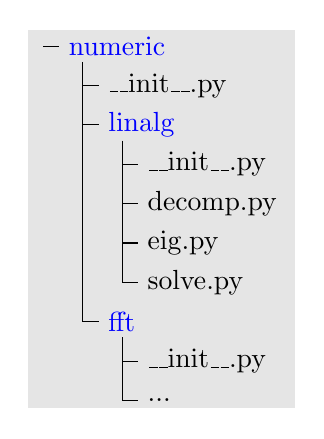
\begin{tikzpicture}
\fill[black!10!white] (-0.2,  0.2) rectangle (3.2, -4.6);
\draw (0.0,  0.0) -- (0.2,  0.0) node[anchor=west] {\color{blue}numeric};
\draw (0.5, -0.2) -- (0.5, -3.5);
\draw (0.5, -0.5) -- (0.7, -0.5) node[anchor=west] {\_\_init\_\_.py};
\draw (0.5, -1.0) -- (0.7, -1.0) node[anchor=west] {\color{blue}linalg};
\draw (1.0, -1.2) -- (1.0, -3.0);
\draw (1.0, -1.5) -- (1.2, -1.5) node[anchor=west] {\_\_init\_\_.py};
\draw (1.0, -2.0) -- (1.2, -2.0) node[anchor=west] {decomp.py};
\draw (1.0, -2.5) -- (1.2, -2.5) node[anchor=west] {eig.py};
\draw (1.0, -3.0) -- (1.2, -3.0) node[anchor=west] {solve.py};
\draw (0.5, -3.5) -- (0.7, -3.5) node[anchor=west] {\color{blue}fft};
\draw (1.0, -3.7) -- (1.0, -4.5);
\draw (1.0, -4.0) -- (1.2, -4.0) node[anchor=west] {\_\_init\_\_.py};
\draw (1.0, -4.5) -- (1.2, -4.5) node[anchor=west] {...};
\end{tikzpicture}
\end{column}
\begin{column}{7.3cm}
In jedem Paket-Ordner: \lstinline{__init__.py} \\
(kann leer sein)
\vspace{2mm}
\begin{lstlisting}[style=Python]
import numeric
numeric.foo() #Aus __init__.py
numeric.linalg.eig.foo()
\end{lstlisting}
\begin{lstlisting}[style=Python]
from numeric.linalg import eig
eig.foo()
\end{lstlisting}
\end{column}
\end{columns}
\end{frame}

%%% Local Variables: 
%%% mode: latex
%%% latex-run-command: pdflatex
%%% TeX-master: "vortrag"
%%% End: 

\section*{Ausnahmen}
\begin{aufgabe}
Lesen Sie vom Benuter eine Zahl ein und geben Sie ihr Quadrat aus. Was passiert, wenn der Benutzer etwas anderes als eine Zahl eingibt? Geben Sie eine benutzerfreundliche Fehlermeldung aus!
\end{aufgabe}

\begin{aufgabe}[Fakult"at erweitert]
Die Fakult"at ist nur f"ur nat"urliche Zahlen definiert. Wie reagiert die Funktion aus Aufgabe \ref{fakultaet} auf negative Parameter? Lassen Sie die Funktion in diesem Fall einen \texttt{ValueError} ausl"osen.
\end{aufgabe}

\begin{aufgabe}Schreiben Sie ein Programm, welches in einer Endlosschleife Eingaben vom Benutzer einliest und jeweils pr"uft, ob die Eingabe ein Palindrom ist (verwenden Sie die Funktion aus Aufgabe \ref{palindrom}). 

Was passiert, wenn der Benutzer \texttt{Ctrl-C} oder \texttt{Ctrl-D} dr"uckt? "Andern Sie das Programm, sodass der Benutzer beim Dr"ucken von \texttt{Ctrl-C} oder \texttt{Ctrl-D} gefragt wird, ob er das Programm beenden m"ochte.
\end{aufgabe}

\begin{aufgabe}
Mit dem Modul \texttt{readline} k"onnen f"ur die Benutzereingaben mittels \texttt{raw\_input} Editierm"oglichkeiten wie in der Shell aktiviert werden. Dieses Modul ist standardm"a"sig nur unter *nix-Systemen verf"ugbar. Folgender Code importiert das Modul nicht auf Windows-Rechnern:
\begin{lstlisting}
if not sys.platform.startswith("win"):
    import readline
    import rlcompleter
    readline.parse_and_bind("tab: complete")
\end{lstlisting}
Warum ist ein Ansatz mit Ausnahmen besser? Schreiben Sie den Code so um, dass er mit Ausnahmen arbeitet.
\end{aufgabe}

%%% Local Variables: 
%%% mode: latex
%%% TeX-master: "uebung1"
%%% End: 


\vielspass

\part{Teil 2}
\section*{Datentypen II}

\begin{aufgabe}
Die h"aufigsten Buchstaben im deutschen Alphabet sind A, D, E, H, I, N, R, S, T, U. Schreiben Sie eine Funktion, welche testet, ob ein String auschlie"slich aus solchen Buchstaben besteht.
\begin{teilaufgabe}
Wie kann man die Funktion unabh"angig von Gro"s-/Kleinschreibung machen?
\end{teilaufgabe}
\begin{teilaufgabe}
Wie bekommt man die Buchstaben des "ubergebenen Strings heraus, die nicht in den h"aufigsten Buchstaben enthalten sind?
\end{teilaufgabe}
\end{aufgabe}


\begin{aufgabe}[Morsecode]
Schreiben Sie eine Funktion, welche Strings in Morsecode "ubersetzt. Die "Ubersetzung soll unabh"angig sein von Gro"s-/Kleinschreibung.

\begin{tabular}[h]{|l|ll|l|ll|l|l|}
\hline
A&$\cdot$ --&&J&$\cdot$ -- -- --&&S&$\cdot$ $\cdot$ $\cdot$\\
B&-- $\cdot$ $\cdot$ $\cdot$&&K&-- $\cdot$ --&&T&--\\
C&-- $\cdot$ -- $\cdot$&&L&$\cdot$ -- $\cdot$ $\cdot$&&U&$\cdot$ $\cdot$ --\\
D&-- $\cdot$ $\cdot$&&M&-- --&&V&$\cdot$ $\cdot$ $\cdot$ --\\
E&$\cdot$&&N&-- $\cdot$&&W&$\cdot$ -- --\\
F&$\cdot$ $\cdot$ -- $\cdot$&&O&-- -- --&&X&-- $\cdot$ $\cdot$ --\\
G&-- -- $\cdot$&&P&$\cdot$ -- -- $\cdot$&&Y&-- $\cdot$ -- --\\
H&$\cdot$ $\cdot$ $\cdot$ $\cdot$&&Q&-- -- $\cdot$ --&&Z&-- -- $\cdot$ $\cdot$\\
I&$\cdot$ $\cdot$&&R&$\cdot$ -- $\cdot$&&&\\
\hline
\end{tabular}
\end{aufgabe}


\section{Object Oriented Programming}

\begin{frame}{Object Oriented Programming}
\begin{itemize}
\item So far: \alert{procedural programming}
\begin{itemize}
\item Data
\item Functions taking data as parameters and returning results
\end{itemize}
\item Alternative: Group data and functions belonging together to form \alert{custom data types}
\item $\rightarrow$ Extensions of structures in C/Fortran
\end{itemize}
\end{frame}

\begin{frame}[fragile]{Using Simple Classes as Structs}
\begin{lstlisting}[style=Python]
class Point:
    pass

p = Point()
p.x = 2.0
p.y = 3.3
\end{lstlisting}
\begin{itemize}
\item \alert{Class}: Custom date type (here: \texttt{Point})
\item \alert{Object}: Instance of a class (here: \texttt{p})
\item Attributes (here \texttt{x}, \texttt{y}) can be added dynamically
\end{itemize}
\end{frame}

\begin{frame}[fragile]{Classes}
\begin{lstlisting}[style=Python]
class Point:
    def __init__(self, x, y):
        self.x = x
        self.y = y

p = Point(2.0, 3.0)
print p.x, p.y
p.x = 2.5
p.z = 42
\end{lstlisting}
\begin{itemize}
\item \texttt{\_\_init\_\_}: Is called automatically after creating an object
\end{itemize}
\end{frame}

\begin{frame}[fragile]{Methods on Objects}
\begin{lstlisting}[style=Python]
class Point:
    def __init__(self, x, y):
        self.x = x
        self.y = y

    def norm(self):
        n = math.sqrt(self.x**2 + self.y**2)
        return n

p = Point(2.0, 3.0)
print p.x, p.y, p.norm()
\end{lstlisting}
\begin{itemize}
\item Method call: automatically sets the object as first parameter
\item $\rightarrow$ traditionally called \lstinline{self}
\item\alert{Careful}: Overloading of methods not possible!
\end{itemize}
\end{frame}

\begin{frame}[fragile]{Converting Objects to Strings}
\onslide<1->
Default return value of \lstinline{str(...)} for objects of custom classes:
\begin{lstlisting}[style=Shell]
>>> p = Point(2.0, 3.0)
>>> print p  # --> print str(p)
<__main__.Point instance at 0x402d7a8c>
\end{lstlisting}
\vspace{2mm}

\onslide<2->
This behaviour can be overwritten:
\begin{lstlisting}[style=Python]
def __str__(self):
    return "(%i, %i)" % (self.x, self.y)
\end{lstlisting}
\begin{lstlisting}[style=Shell]
>>> print p
(2, 3)
 \end{lstlisting}
\end{frame}

\begin{frame}[fragile]{Comparing Objects}
\onslide<1->
Default: \texttt{==} checks for object identity of custom objects.
\begin{lstlisting}[style=Shell]
>>> p1 = Point(2.0, 3.0)
>>> p2 = Point(2.0, 3.0)
>>> p1 == p2
False
\end{lstlisting}
%\vspace{2mm}
\onslide<2->
This behaviour can be overwritten:
\begin{lstlisting}[style=Python]
def __eq__(self, other):
    return (self.x == other.x) and
           (self.y == other.y)
\end{lstlisting}
\begin{lstlisting}[style=Shell]
>>> p1 == p2 # Check for equal values
True
>>> p1 is p2 # Check for identity
False
\end{lstlisting}
\end{frame}

\begin{frame}[fragile]{Comparing Objects}
More relational operators:
\begin{itemize}
\item \texttt{<} : \lstinline{__lt__(self, other)}
\item \texttt{<=} : \lstinline{__le__(self, other)}
\item \texttt{!=} : \lstinline{__ne__(self, other)}
\item \texttt{>} : \lstinline{__gt__(self, other)}
\item \texttt{>=} : \lstinline{__ge__(self, other)}
\end{itemize}
\vspace{2mm}
Alternative: \lstinline{__cmp__(self, other)}, returns:
\begin{itemize}
\item negative integer when \lstinline{self < other}
\item zero when \lstinline{self == other}
\item positive integer when \lstinline{self > other}
\end{itemize}
\end{frame}

\begin{frame}{Emulating Existing Data Types}
Classes can emulate built-in data types:
\begin{itemize}
\item Numbers: arithmetics, \texttt{int(myobj)}, \texttt{float(myobj)}, \dots
\item Functions: \texttt{myobj(...)}
\item Sequences: \texttt{len(myobj)}, \texttt{myobj[...]}, \lstinline{x in myobj}, ...
\item Iterators: \lstinline{for i in myobj}
\end{itemize}
\vspace{2mm}
See documentation:\\
\href{http://docs.python.org/ref/specialnames.html}{http://docs.python.org/ref/specialnames.html}
\end{frame}

\begin{frame}[fragile]{Class Variables}
Have the same value for all instances of a class:
\begin{lstlisting}[style=Python]
class Point:
    count = 0  # Count all point objects
    def __init__(self, x, y):
        self.__class__.count += 1
        ...
\end{lstlisting}
\begin{lstlisting}[style=Shell]
>>> p1 = Point(2, 3); p2 = Point(3, 4)
>>> p1.count
2
>>> p2.count
2
>>> Point.count
2
\end{lstlisting}
\end{frame}

\begin{frame}[fragile]{Class Methods and Static Methods}
\begin{lstlisting}[style=Python]
class Spam:
    spam = "I don't like spam."

    @classmethod
    def cmethod(cls):
        print cls.spam
       
    @staticmethod
    def smethod():
        print "Blah blah."
\end{lstlisting}
\begin{lstlisting}[style=Python]
Spam.cmethod()
Spam.smethod()
s = Spam()
s.cmethod()
s.smethod()
\end{lstlisting}
\end{frame}

\begin{frame}{Inheritance}
There are often classes that are very similar to each other.\\
\alert{Inheritance} allows for:
\begin{itemize}
\item Hierarchical class structure (is-a-relationship)
\item Reusing of similar code
\end{itemize}
\vspace{5mm}
Example: Different types of phones
\begin{itemize}
\item Phone
\item Mobile phone (is a phone with additional functionality)
\item Smart phone (is a mobile phone with additional functionality)
\end{itemize}
\end{frame}

\begin{frame}[fragile]{Inheritance}
\begin{lstlisting}[style=Python]
class Phone:
    def call(self):
        pass

class MobilePhone(Phone):
    def send_text(self):
        pass
\end{lstlisting}
MobilePhone now inherits methods and attributes from Phone.
\begin{lstlisting}[style=Python]
h = MobilePhone()
h.call() # inherited from Phone
h.send_text() # own method
\end{lstlisting}
\end{frame}

\begin{frame}[fragile]{Overwriting Methods}
Methods of the parent class can be overwritten in the child class:
\begin{lstlisting}[style=Python]
class MobilePhone(Phone):
    def call(self):
        find_signal()
        Phone.call(self)
\end{lstlisting}
\end{frame}

\begin{frame}[fragile]{Multiple Inheritance}
Classes can inherit from multiple parent classes. Example:
\begin{itemize}
\item SmartPhone is a mobile phone
\item SmartPhone is a camera
\end{itemize}
\begin{lstlisting}[style=Python]
class SmartPhone(MobilePhone, Camera)
    pass

h = SmartPhone()
h.call()  # inherited from MobilePhone
h.take_photo() # inherited from Camera
\end{lstlisting}
Attributes are searched for in the following order:

SmartPhone, MobilePhone, parent class of MobilePhone (recursively), Camera, parent class of Camera (recursively).
\end{frame}

\begin{frame}[fragile]{Private Attributes}
\begin{itemize}
\item There are no private variables or private methods in Python.
\item \alert{Convention:} Mark attributes that shouldn't be accessed from outside with an underscore: \lstinline{_foo}.
\item To avoid name conflicts during inheritance: Names of the form \lstinline{__foo} are replaced with \lstinline{_classname__foo}:
\end{itemize}
\begin{lstlisting}[style=Python]
class Spam:
    __eggs = 3
\end{lstlisting}
\begin{lstlisting}[style=Shell]
>>> dir(Spam)
>>> ['_Spam__eggs', '__doc__', '__module__']
\end{lstlisting}
\end{frame}

\begin{frame}[fragile]{Properties}
If certain actions (checks, conversions) are to be executed while accessing attributes, use \alert{getter} and \alert{setter}:
\begin{lstlisting}[style=Python]
class Spam(object):
    def __init__(self):
        self._value = 0
    
    def get_value(self):
        return self._value

    def set_value(self, value):
        if value <= 0:  self._value = 0
        else:  self._value = value

    value = property(get_value, set_value)
\end{lstlisting}
\end{frame}

\begin{frame}[fragile]{Properties}
Properties can be accessed like any other attributes:
\begin{lstlisting}[style=Shell]
>>> s = Spam()
>>> s.value = 6   # set_value(6)
>>> s.value       # get_value()
>>> 6
>>> s.value = -6  # set_value(-6)
>>> s.value       # get_value()
>>> 0
\end{lstlisting}
\begin{itemize}
\item Getter and setter can be added later without changing the API
\item Access to \lstinline{_value} still possible
\end{itemize}

\end{frame}



\section*{Pythons Standardbibliothek}

\begin{aufgabe}[Passwort-Generator]
Schreiben Sie ein Programm, welches ein acht Zeichen langes Passwort generiert. \hinweis Schauen Sie sich \lstinline{string.letters} und \lstinline{string.digits} an!
\end{aufgabe}

\begin{aufgabe}
Schreiben Sie ein Programm, welches alle Dateien eines Verzeichnisses mit Endung \texttt{htm} umbenennt, sodass die neue Endung \texttt{html} lautet.
\end{aufgabe}

\begin{aufgabe}[CSV]
Gegeben sei folgende Daten-Datei:
\begin{verbatim}
"Mr. Spock","Vulcan"
"Freddie ""Nightmare"" Krueger, Jr.","Elm Street 42,
Springfield" 
\end{verbatim}
(Der Zeilenumbruch im zweiten Datensatz ist gewollt!). Die Datens"atze bestehen aus zwei Feldern, Name und Adresse. Lesen sie alle Datens"atze ein und geben Sie sie auf dem Bildschirm aus.

\hinweis Diesen Datensatz m"ochte man nicht selbst parsen. (Warum?)
\end{aufgabe}

\begin{aufgabe}[Spa"s mit regul"aren Ausdr"ucken]
Schreiben Sie ein Programm, welches alle html-Tags aus einer html-Datei entfernt. (html-Tags sind in spitzen Klammern eingeschlossen, also z.B. \texttt{<body>}, \texttt{</body>}.)
\end{aufgabe}

\begin{aufgabe}[Einweg-Chat]
Schreiben Sie einen einfachen \glqq Chat-Server\grqq{} und \glqq Chat-Client\grqq . Der Server horcht auf eingehende Socket-Verbindungen. Sobald eine Verbindung hergestellt ist, liest der Server die Daten vom Client und gibt sie auf dem Bildschirm aus. Der Client liest Eingaben von der Tastatur und sendet diese an den Server. \glqq Chatten\grqq{} Sie mit Ihrem Nachbarn! 
\end{aufgabe}






\vielspass

\part{Teil 3}
\section{Neues in Python 2.5}

\begin{frame}[fragile]
\frametitle{Conditional Expressions}
Kurze Schreibweise f"ur bedingte Zuweisung. Statt:
\begin{lstlisting}
if zahl<0:
    s = "Negativ"
else:
    s = "Positiv"
\end{lstlisting}
kann man schreiben:
\begin{lstlisting}
s = "Negativ" if zahl<0 else "Positiv"
\end{lstlisting}
\end{frame}

\begin{frame}[fragile]
\frametitle{Das \texttt{with}-Statement}
Einige Objekte bieten Kontext-Management an. Damit k"onnen \lstinline{try... finally}\,-Bl"ocke einfacher geschrieben werden:
\begin{lstlisting}
from __future__ import with_statement

with open("test.txt") as f:
    for line in f:
        print line
\end{lstlisting}
Nach dem \lstinline{with}-Block ist das Dateiobjekt stets wieder geschlossen, auch wenn im Block eine Exception auftrat.
\end{frame}

\begin{frame}[fragile]
\frametitle{Partielle Funktionsanwendung}
\begin{lstlisting}
import functools

def add (a, b):
    return a + b

add_ten = functools.partial(add, b=10)
add_ten(42)
\end{lstlisting}
\end{frame}

\section{Flexiblere Funktionen}

\begin{frame}[fragile]
\frametitle{Funktionsparameter aus Listen und Dictionaries}
\begin{lstlisting}
def spam(a, b, c, d):
    print a, b, c, d
\end{lstlisting}
Man kann positionale Parameter aus Listen erzeugen:
\begin{lstlisting}[style=Shell]
>>> args = [3, 6, 2, 3]
>>> spam(*args)
3 6 2 3
\end{lstlisting}
Man kann Keyword-Paramter aus Dictionaries erzeugen:
\begin{lstlisting}[style=Shell]
>>> kwargs = {"c": 5, "a": 2, "b": 4, "d":1}
>>> spam(**kwargs)
2 4 5 1
\end{lstlisting}
\end{frame}

\begin{frame}[fragile]
\frametitle{Funktionen mit beliebigen Parametern}
\begin{lstlisting}
def spam(*args, **kwargs):
    for i in args:
        print i
    for i in kwargs:
        print i, kwargs[i]
\end{lstlisting}
\begin{lstlisting}[style=Shell]
>>> spam(1, 2, c=3, d=4)
1
2
c 3
d 4
\end{lstlisting}
\end{frame}

\begin{frame}[fragile]
\frametitle{Anonyme Funktionen}
\begin{lstlisting}
def make_incrementor(n):
    return lambda x: x + n
\end{lstlisting}
\begin{lstlisting}[style=Shell]
>>> f = make_incrementor(42)
>>> f(0)
42
>>> f(1)
43
\end{lstlisting}
Sinnvoll, wenn einfache Funktionen als Parameter "ubergeben werden sollen.
\end{frame}

\section{Funktionale Techniken mit Listen}

\begin{frame}[fragile]
\frametitle{List Comprehension}
Abk"urzende Schreibweise zum Erstellen von Listen aus for-Schleifen. Statt:
\begin{lstlisting}
a = []
for i in range(10):
    a.append(i**2)
\end{lstlisting}
kann man schreiben:
\begin{lstlisting}
a = [i**2 for i in range(10)]
\end{lstlisting}
\end{frame}

\begin{frame}[fragile]
\frametitle{Map}
Anwenden einer Funktion auf alle Elemente einer Liste:
\begin{lstlisting}[style=Shell]
>>> a = [1.6, 4.0, 81.0, 9.0]
>>> map(math.sqrt, a)
[1.2649110640673518, 2.0, 9.0, 3.0]
>>> map(lambda x: x * 2, a)
[3.2000000000000002, 8.0, 162.0, 18.0]
\end{lstlisting}
Wenn die Funktion mehr als einen Parameter nimmt, kann je zus"atzlichem Parameter eine weitere Liste "ubergeben werden:
\begin{lstlisting}[style=Shell]
>>> map(math.pow, a, [2 for i in a])
[2.5600000000000005, 16.0, 6561.0, 81.0]
\end{lstlisting}
\end{frame} 

\begin{frame}[fragile]
\frametitle{Filter}
Gibt Elemente einer Liste zur"uck, die nach Anwendung einer Funktion wahr sind:
\begin{lstlisting}[style=Shell]
>>> a = [1, 2, 3, 4, 5, 6, 7, 8, 9]
>>> filter(lambda x: x % 2, a)
[1, 3, 5, 7, 9]
\end{lstlisting}
\end{frame}

\begin{frame}[fragile]
\frametitle{Reduce}
Wendet Funktion auf die ersten beiden Elemente an, dann auf das Ergebnis und das n"achste Element etc.
\begin{lstlisting}[style=Shell]
>>> def add(x, y):
...     return x + y
...
>>> a = [1, 2, 3, 4, 5, 6, 7, 8, 9]
>>> reduce(add, a)
45
\end{lstlisting}
Optionaler Startwert, der vor die Liste gesetzt wird:
\begin{lstlisting}[style=Shell]
>>> reduce(add, a, 10)
55
\end{lstlisting}
\end{frame}

\section{Iteratoren, Generatoren, Generator-Audr"ucke}

\begin{frame}[fragile]
\frametitle{Iteratoren}
Was passiert, wenn \lstinline{for} auf einem Objekt aufgerufen wird?
\begin{lstlisting}[style=Python]
for i in obj:
    pass
\end{lstlisting}
\begin{itemize}
\item Auf \lstinline{obj} wird die \lstinline{__iter__}-Methode aufgerufen, welche einen Iterator zur"uckgibt
\item Auf dem Iterator wird bei jedem Durchlauf \lstinline{next()} aufgerufen
\item Eine \lstinline{StopIteration}-Ausnahme beendet die for-Schleife
\end{itemize}
\end{frame}

\begin{frame}[fragile]
\frametitle{Iteratoren}
\begin{lstlisting}[style=Python]
class Reverse:
    def __init__(self, data):
        self.data = data
        self.index = len(data)
    def __iter__(self):
        return self
    def next(self):
        if self.index == 0:
            raise StopIteration
        self.index = self.index - 1
        return self.data[self.index]
\end{lstlisting}
\begin{lstlisting}[style=Shell]
>>> for char in Reverse("spam"):
...     print char,
...
m a p s
\end{lstlisting}
\end{frame}

\begin{frame}[fragile]
\frametitle{Generatoren}
Einfache Weise, Iteratoren zu erzeugen:
\begin{itemize}
\item Werden wie Funktionen definiert
\item \lstinline{yield}-Statement, um Daten zur"uckzugeben und beim n"achsten \lstinline{next}-Aufruf dort weiterzumachen
\end{itemize}
\begin{lstlisting}[style=Python]
def reverse(data):
    for index in range(len(data)-1, -1, -1):
        yield data[index]
\end{lstlisting}
\begin{lstlisting}[style=Shell]
>>> for char in reverse("spam"):
...     print char,
...
m a p s
\end{lstlisting}
\end{frame}

\begin{frame}[fragile]
\frametitle{Generator-Audr"ucke}
"Ahnlich zu List Comprehensions kann man anonyme Iteratoren erzeugen:
\begin{lstlisting}[style=Shell]
>>> data = "spam"
>>> for c in (data[i] for i in
...           range(len(data)-1, -1, -1)):
...     print c,
...
m a p s
\end{lstlisting}
\end{frame}


\section{Etwas Dynamik}
\begin{frame}[fragile]
\frametitle{Dynamische Attribute}
Erinnerung: Man kann Attribute von Objekten zur Laufzeit hinzuf"ugen:
\begin{lstlisting}
class Empty:
    pass

a = Empty()
a.spam = 42
a.eggs = 17
\end{lstlisting}
\vspace{2mm}
Und entfernen:
\begin{lstlisting}
del a.spam
\end{lstlisting}
\end{frame}

\begin{frame}[fragile]
\frametitle{getattr, setattr}
Man kann Attribute von Objekten als Strings ansprechen:
\begin{lstlisting}
import math
f = getattr(math, "sin")
print f(x) # sin(x)
\end{lstlisting}
\vspace{2mm}
\begin{lstlisting}
a = Empty()
setattr(a, "spam", 42)
print a.spam
\end{lstlisting}
N"utzlich, wenn man z.B. Attributnamen aus User-Input oder Dateien liest.
\end{frame}

%%% Local Variables: 
%%% mode: latex
%%% latex-run-command: pdflatex
%%% TeX-master: "vortrag"
%%% End: 

\section{Neues in Python 2.7}

\begin{frame}[fragile]{Neues in Python 2.7}

\begin{itemize}
\item Neue Syntax f"ur Mengen: Statt \texttt{set(1, 2, 3)} kann man schreiben: \texttt{\{1,2,3}\}
\item Analog zu List Comprehensions gibt es Set Comprehensions und Dictionary Comprehensions zum schnellen Erzeugen:
\begin{lstlisting}
s = {i*2 for in in range(3)}
d = {i: i*2 for i in range(3)}
\end{lstlisting}
\item \texttt{collections.OrderedDict}: Beim normalen Dictionary haben die Eintr"age eine willk"urliche Reihenfolge. OrderedDict kann die Eintr"age sortiert hinzuf"ugen.
\end{itemize}

\end{frame}

\section*{wxPython}

\begin{aufgabe}[Hello World]
\label{aufg-hello-world}Programmieren Sie die Hello-World-Anwendung aus der Vorlesung, welche ein leeres Frame erzeugt. Probieren Sie verschiedene Parameter f"ur Titel, Gr"o\3e und Position des Frames.
\end{aufgabe}

\begin{aufgabe}[Statischer Text]
\begin{teilaufgabe}
Erweitern Sie das Programm aus Aufgabe \ref{aufg-hello-world}, sodass es Text im Frame darstellt (\lstinline{wx.StaticText}). Stellen Sie mehrzeiligen Text zentriert, linsb"undig, rechtsb"undig dar.
\end{teilaufgabe}
\begin{teilaufgabe}
F"ugen Sie mehrere \lstinline{wx.StaticText}-Widgets in das Frame ein. Was passiert, wenn Sie keine Positionsangaben machen? Ordnen Sie die Widgets mit Positionsangaben an. Beobachten Sie das Verhalten, wenn das Frame in seiner Gr"o\3e ver"andert wird.
\end{teilaufgabe}
\end{aufgabe}


\begin{aufgabe}[Buttons]
\begin{teilaufgabe}
Erweitern Sie das Programm aus Aufgabe \ref{aufg-hello-world}, sodass es einen Button darstellt. Wird auf diesen Button geclickt, soll sich das Programm beenden. (Dazu das MainFrame schlie\3en: \lstinline{self.Close(True)})
\end{teilaufgabe}
\begin{teilaufgabe}
F"ugen Sie weitere Buttons hinzu. Die Buttons sollen verschiedene Aktionen ausf"uren (z.B. verschiedenen Text im Terminal ausgeben), solabld sie geclickt werden.
\end{teilaufgabe}
\end{aufgabe}

\begin{aufgabe}[Sizer]
\label{aufg-sizer}
Erstellen Sie ein Frame mit einem BoxSizer und Buttons und probieren Sie verschiedene M"oglichkeiten des BoxSizers aus. Z.B.:
\begin{itemize}
\item Ein Button, welcher stets so gro\3 wie das gesamte Frame ist
\item Mehrere Buttons nebeneinander
\item Mehrere Buttons untereinander
\end{itemize}
Sie brauchen die Buttons nicht mit Funktionen belegen, hier geht es allein um das Layout.
\end{aufgabe}


\begin{aufgabe}[RadioBox]
\label{aufg-radiobox}
Erstellen Sie ein Frame, welches eine RadioBox darstellt. Sobald der Anwender ein Item ausw"ahlt, soll die Auswahl in der Konsole ausgegeben werden.

\hinweis Im Gegensatz zu den bisherigen Aufgaben ist es nun notwendig, das RadioBox-Objekt zu einem Objekt-Attriut des MainFrames zu machen, damit sie auch au"serhalb der init-Methode des Frames darauf zugreifen k"onnen: \lstinline{self.radiobox = ...}
\end{aufgabe}

\begin{aufgabe}[Text-Editor]
Schreiben Sie einen einfachen Text-Editor. Gehen Sie dabei wie folgt vor:
\begin{teilaufgabe}[Texteingabe-Feld]
Erstellen Sie ein Frame mit einem mehrzeiligen TextCtrl-Widget. Das Textfeld sollte das ganze Frame ausf"ullen, vgl. Aufgabe \ref{aufg-sizer}. Probieren Sie die Nutzung des Widgets aus!
\begin{itemize}
\item Was passiert, wenn Sie sehr viele Zeilen in das Widget einf"ugen, oder sehr lange Zeilen?
\item Was bewirken Tastenkombinatioen wie Ctrl-C, Ctrl-V, Ctrl-X, Einfg, Entf, \dots?
\end{itemize}
\end{teilaufgabe}
\begin{teilaufgabe}[Men"us]
F"ugen Sie eine Men"uzeile hinzu und ein Men"u \glqq File\grqq. Das File-Men"u soll den Eintrag \glqq Quit\grqq{} enthalten.
\end{teilaufgabe}
\begin{teilaufgabe}[Statuszeile]
F"ugen Sie eine Statuszeile hinzu. Beobachten Sie, wir dort die Hilfetexte der Men"ueintr"age angezeigt werden.
\end{teilaufgabe}
\begin{teilaufgabe}[Neue Datei]
F"ugen Sie dem File-Men"u einen Eintrag \glqq New\grqq{} hinzu, welcher den Inhalt des Texteingabe-Feldes l"oscht.

\hinweis Analog zu Aufgabe \ref{aufg-radiobox} ist es nun notwendig, das Textfeld zu einem Objektattribut des MainFrame-Objekts zu machen.
\end{teilaufgabe}
\begin{teilaufgabe}[Datei "offnen]
F"ugen Sie dem File-Men"u einen Eintrag \glqq Open\dots\grqq{} hinzu. "Uber einen FileDialog soll der Anwender eine Datei ausw"ahlen k"onnen, welche im Textfeld angezeigt wird.
\end{teilaufgabe}

\begin{teilaufgabe}[Datei speichern als]
F"ugen Sie dem File-Men"u einen Eintrag \glqq Save as\dots\grqq{} hinzu. "Uber einen FileDialog soll der Anwender eine Datei ausw"ahlen k"onnen, in welcher der Inhalt des Textfelds gespeichert wird.
\end{teilaufgabe}

\begin{teilaufgabe}[Datei speichern]
F"ugen Sie dem File-Men"u einen Eintrag \glqq Save\grqq{} hinzu, der die Datei unter dem Namen speichert, unter dem sie ge"offnet bzw. zuletzt gespeichert wurde. Geben Sie daf"ur dem MainFrame z.B. ein Objekt-Attribut \lstinline{filename}, welches bei den Aktionen \glqq Save as\dots\grqq{} und \glqq Open \dots\grqq{} entsprechend gesetzt wird.

Achtung, es gibt nicht immer einen Dateinamen, wenn der Anwender speichern will! (Wann?) In einem solchen Fall sollte das \lstinline{filename}-Attribut \lstinline{None} sein; idealerweise wird dann bei \glqq Save\grqq{} ebenfalls ein FileDialog angeboten.

Des weiteren kann man den Dateinamen in der Titelzeile des Frames anzeigen lassen (\lstinline{SetTitle}).
\end{teilaufgabe}

\begin{teilaufgabe}[Anzeige in der Statuszeile]
Lassen Sie die Aktionen, die das Programm ausf"uhrt, in der Statuszeile anzeigen, z.B. \glqq File bla.txt saved.\grqq
\end{teilaufgabe}

\begin{teilaufgabe}[Speicherstatus]
Speichern Sie den Status, ob eine Datei seit dem "Offnen oder dem letzten Speichern ge"andert wurde, in einem Attribut des MainFrame-Objekets. Lassen Sie den Status in geeigneter Weise in der Titelleiste des Frames anzeigen. Das Event, welches das TextCtrl beim "Andern des Textes ausgel"ost, ist \lstinline{wx.EVT_TEXT}.

Zus"atzlich k"onnte man Warnungen (z.B. MessageDialog) einf"ugen, wenn der Anwender bei einer ungespeicherten Datei \glqq Open\dots\grqq, \glqq Quit\grqq{} oder \glqq New\grqq{} ausf"uhren m"ochte.
\end{teilaufgabe}

\end{aufgabe}


\section{Zusammenfassung und Ausblick}

\begin{frame}{Zusammenfassung}
Wir haben kennengelernt:
\begin{itemize}
\item verschiedene \alert{Datentypen} (tw. \glqq High Level\grqq)
\item die wichtigsten \alert{Statements}
\item \alert{Funktion}sdeklaration und -Benutzung
\item \alert{Module} und Pakete
\item Fehler und \alert{Ausnahmen}, Behandlung selbiger
\item \alert{objektorientierte Programmierung}
\item einige h"aufig verwendete Standardmodule
\end{itemize}
\end{frame}

\begin{frame}{Offene Punkte}
Nicht behandelte, tw. fortgeschrittene Themen:
\begin{itemize}
\item Closures, Dekoratoren (Funktionswrapper)
\item Metaklassen
\item Weitere Standardmodule: Mail, WWW, XML, Zeit\&Datum, \dots $\rightarrow$~\href{http://docs.python.org/lib/modindex.html}{http://docs.python.org/lib/modindex.html}
\item Profiling, Debugging, Unittesting
\item Extending und Embedding: Python \& C/C++ $\rightarrow$~\href{http://docs.python.org/ext/ext.html}{http://docs.python.org/ext/ext.html}
\item Third Party-Module: Grafik, Webprogrammierung, Datenbanken, \dots $\rightarrow$~\href{http://pypi.python.org/pypi}{http://pypi.python.org/pypi}
\end{itemize}
\end{frame}

\begin{frame}{Web-Programmierung}
\begin{itemize}
\item CGI-Scripte: Modul \texttt{cgi} aus  Standardbibliothek
\item Webframeworks: Django, TurboGears, Pylons, \dots
\item Templatesysteme: Cheetah, Genshi, Jinja, \dots
\item Content Management Systeme (CMS): Zope, Plone, Skeletonz, \dots
\item Wikis: MoinMoin, \dots
\end{itemize}

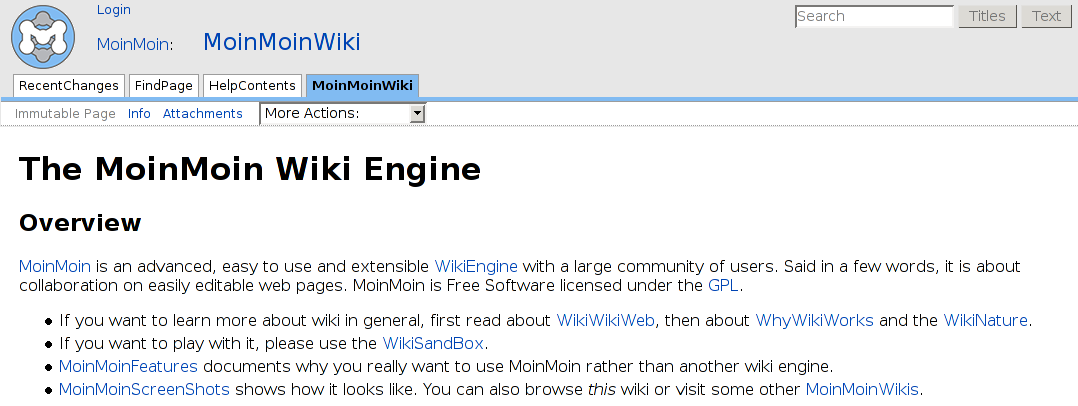
\includegraphics[height=4cm]{images/moinmoin.png}
\end{frame}

\begin{frame}[fragile]{NumPy + SciPy + Matplotlib = Pylab}
Ein Ersatz f"ur MatLab: Matritzenrechnung, numerische Funktionen, Plotten, ...

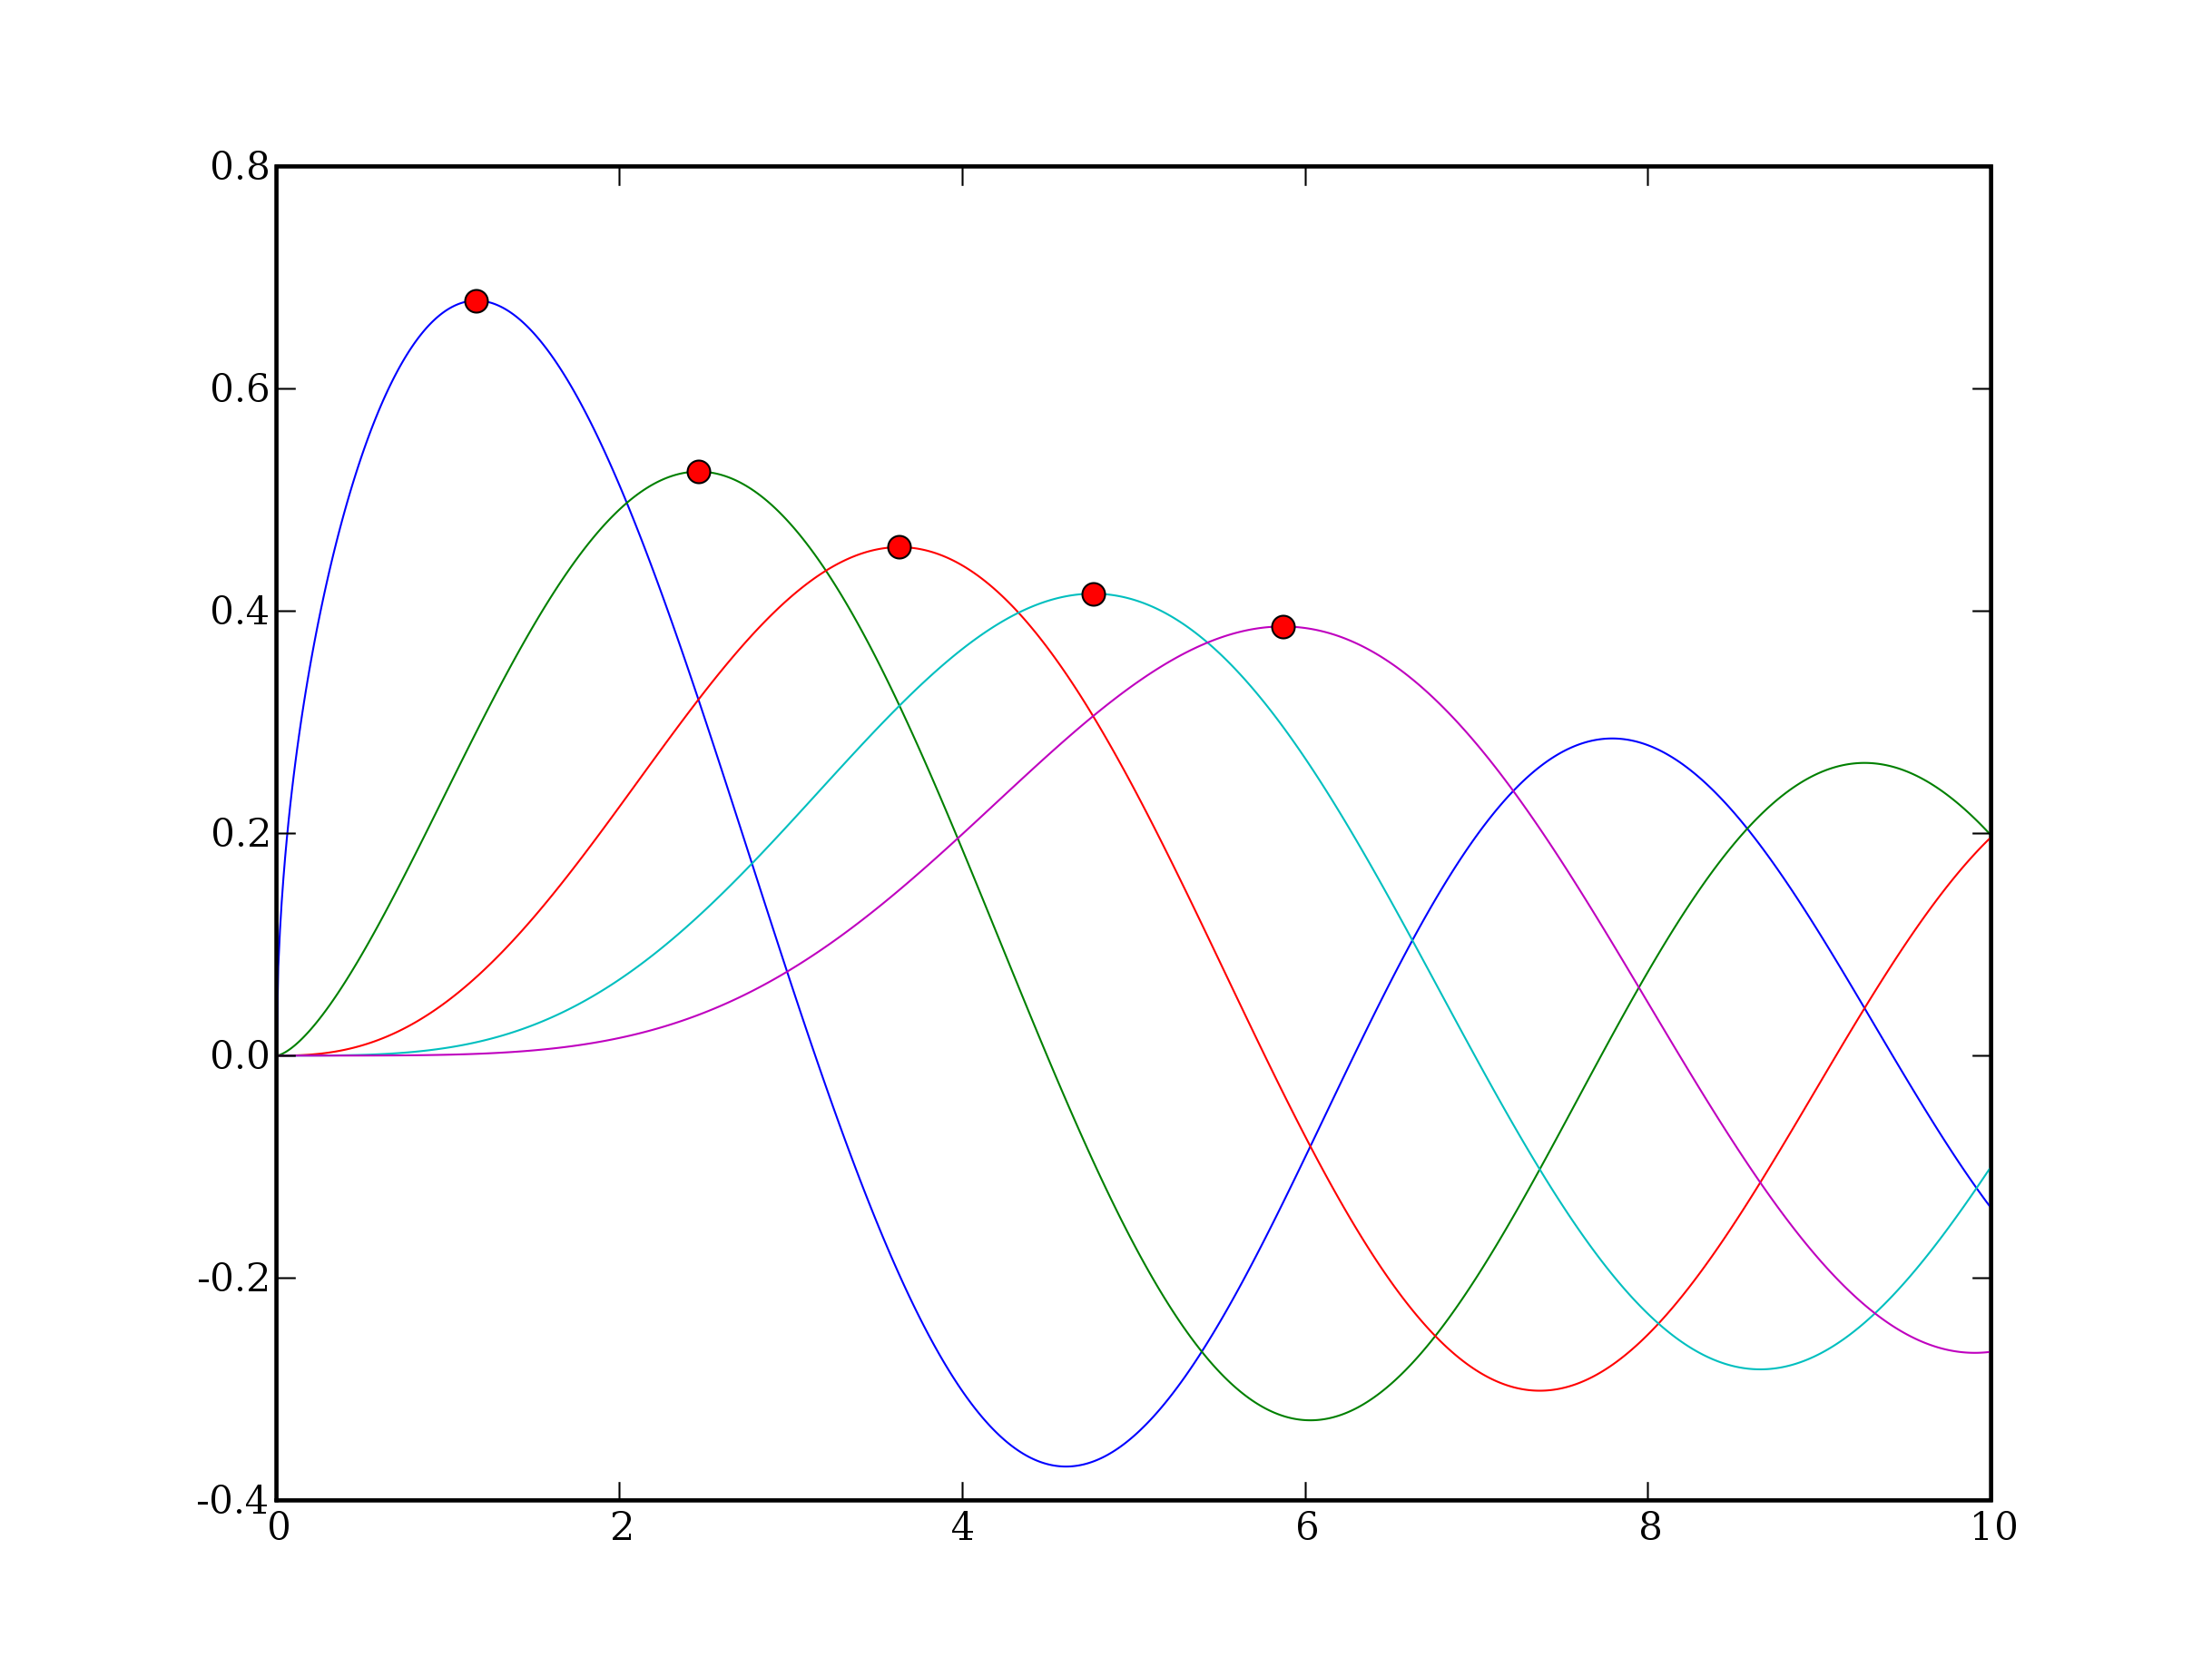
\includegraphics[height=4cm]{images/matplotlib.png}
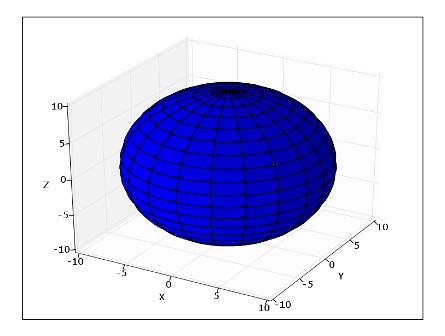
\includegraphics[height=4cm]{images/surface.jpg}

\begin{lstlisting}[style=Python, basicstyle=\small]
A = matrix([[1, 2], [2, 1]]); b = array([1, -1])
matshow(A)
(eigvals, eigvecs) = eig(A)
x = linalg.solve(A, b)
\end{lstlisting}
\end{frame}

\begin{frame}[fragile]{Und mehr...}
\begin{itemize}
\item \alert{ipython}: Eine komfortablere Python-Shell
\item Python und andere Programmiersprachen:
\begin{itemize}
\item Jython: Python-Code in der Java VM ausf"uhren
\item Ctypes: C-Libraries mit Python ansprechen (ab 2.5 in der stdlib)
\item SWIG: C- und C++ -Libraries mit Python ansprechen
\end{itemize}
\item \alert{PIL}: Python Imaging Library f"ur Bildmanipulation
\item \alert{SQLAlchemy}: ORM-Framework
\begin{itemize}
\item Abstraktion: Objektorientierter Zugriff auf DB-Daten
\end{itemize}
\end{itemize}
\end{frame}


\begin{frame}{PyCologne}
\begin{columns}
\begin{column}{0.4\textwidth}
  
\includegraphics[height=5cm]{images/pycologne7.pdf}
\end{column}
\begin{column}{0.6\textwidth}
  \alert{PyCologne}: Python User Group K\"oln
  \begin{itemize}
    \item Trifft sich jeden zweiten Mittwoch im Monat am Rechenzentrum der Uni K\"oln
    \item URL: \href{http://wiki.python.de/pyCologne}{http://wiki.python.de/pyCologne}
  \end{itemize}
\end{column}
\end{columns}
  
\end{frame}


\vielspass

\end{document}

